% !TeX root = priorities.tex
\documentclass[main.tex]{subfiles}

\begin{document}

\section{Priority CP}
\usingnamespace{pcp}

\begin{figure}[t]
  \centering
  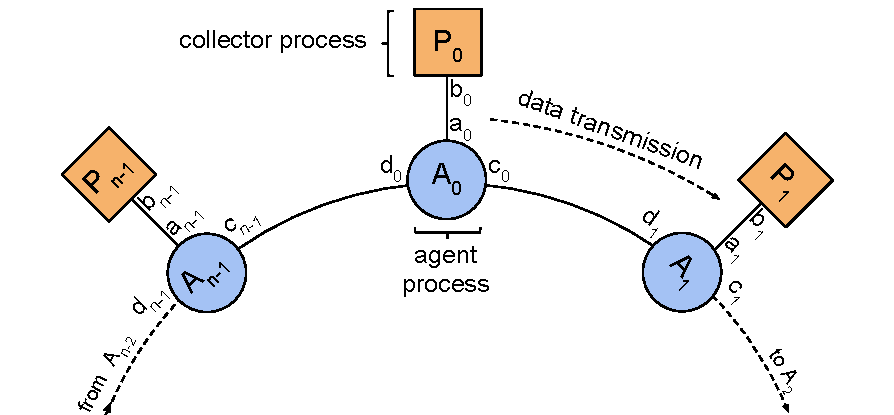
\includegraphics[width=0.8\columnwidth]{scheduler}
  \vspace{-4mm}
  \caption{Cyclic Scheduler from \cite{dardhagay18}}
  \label{fig:scheduler}
  \vspace{-4mm}
  \end{figure}

\subsection{Syntax}

We present an updated version of Priority CP~\cite[PCP]{dardhagay18}, which is Wadler's Classical Processes~\cite[CP]{wadler12} with \emph{priorities}.
The main difference with respect to PCP by Dardha and Gay \cite{dardhagay18} is moving away from a reduction strategy based on cycle elimination using commuting conversions, and towards a reduction strategy using structural congruence.

\paragraph*{Priorities, types, and environments}
Types are based on classical linear logic propositions, and are annotated with priorities ranging over $\cs{o}\in\mathbb{N}$. We let $\ty{A}, \ty{B}, \ty{C}$ range over types, produced by the following grammar.
\[
\begin{array}{lcl}
  \ty{A}, \ty{B}, \ty{C}
  & \coloneqq & \ty{\tytens[\cs{o}]{A}{B}}
    \sep        \ty{\typarr[\cs{o}]{A}{B}}
    \sep        \ty{\tyone[\cs{o}]}
    \sep        \ty{\tybot[\cs{o}]}
    \sep        \ty{\typlus[\cs{o}]{A}{B}}
    \sep        \ty{\tywith[\cs{o}]{A}{B}}
    \sep        \ty{\tynil[\cs{o}]}
    \sep        \ty{\tytop[\cs{o}]}
\end{array}
\]
The types $\ty{\tytens[\cs{o}]{A}{B}}$ and $\ty{\typarr[\cs{o}]{A}{B}}$ type the endpoints of a channel over which we send or receive a channel of type $\ty{A}$, and then proceed as type $\ty{B}$.
The types $\ty{\tyone[\cs{o}]}$ and $\ty{\tybot[\cs{o}]}$ type the endpoints of a channel whose session has terminated, and over which we send or receive a \emph{ping} before closing the channel. These two types act as units for $\ty{\tytens[\cs{o}]{A}{B}}$ and $\ty{\typarr[\cs{o}]{A}{B}}$, respectively.

The types $\ty{\typlus[\cs{o}]{A}{B}}$ and $\ty{\tywith[\cs{o}]{A}{B}}$ type the endpoints of a channel over which we can receive or send a choice between two branches $\ty{A}$ or $\ty{B}$. We have opted for a simplified version of choice and followed the original Wadler's CP \cite{wadler12}, however types $\oplus$ and $\with$ can be trivially generalised to $\ty{\oplus^{\cs{o}}\{l_i:A_i\}_{i\in I}}$ and $\ty{\with^{\cs{o}}\{l_i:A_i\}_{i\in I}}$, respectively as in the original PCP \cite{dardhagay18}.
The types $\ty{\tynil[\cs{o}]}$ and $\ty{\tytop[\cs{o}]}$ type the endpoints of a channel over which we can send or receive a choice between \emph{no options}. These two types act as units for $\ty{\typlus[\cs{o}]{A}{B}}$ and $\ty{\tywith[\cs{o}]{A}{B}}$, respectively.

A typing context $\ty\Gamma$ is a partial function associating channel names to types.
\[
\begin{array}{lcl}
  \ty{\Gamma}, \ty{\Delta}
  & \coloneqq & \ty{\emptyenv}
    \sep        \ty{\Gamma}, \tmty{x}{A}
\end{array}
\]
Duality on types is an involutive function which preserves the priorities of types.
\[
\begin{array}{lcl}
  \ty{\co{(\tyone[\cs{o}])}} & = & \ty{\tybot[\cs{o}]} \\
  \ty{\co{(\tybot[\cs{o}])}} & = & \ty{\tyone[\cs{o}]} \\
  \ty{\co{(\tynil[\cs{o}])}} & = & \ty{\tytop[\cs{o}]} \\
  \ty{\co{(\tytop[\cs{o}])}} & = & \ty{\tynil[\cs{o}]}
\end{array}
\qquad
\begin{array}{lcl}
  \ty{\co{(\tytens[\cs{o}]{A}{B})}} & = & \ty{\typarr[\cs{o}]{\co{A}}{\co{B}}} \\
  \ty{\co{(\typarr[\cs{o}]{A}{B})}} & = & \ty{\tytens[\cs{o}]{\co{A}}{\co{B}}} \\
  \ty{\co{(\typlus[\cs{o}]{A}{B})}} & = & \ty{\tywith[\cs{o}]{\co{A}}{\co{B}}} \\
  \ty{\co{(\tywith[\cs{o}]{A}{B})}} & = & \ty{\typlus[\cs{o}]{\co{A}}{\co{B}}}
\end{array}
\]
The function $\pr(\cdot)$ returns the priority of a type. The function $\minpr(\cdot)$ returns the \emph{minimum} priority of all types a typing context.
\[
\begin{array}{lclclcl}
  \pr(\ty{\tyone[\cs{o}]})        & = & \cs{o}  \\
  \pr(\ty{\tybot[\cs{o}]})        & = & \cs{o}  \\
  \pr(\ty{\tynil[\cs{o}]})        & = & \cs{o}  \\
  \pr(\ty{\tytop[\cs{o}]})        & = & \cs{o}  \\
  \\
  \minpr(\ty{\emptyenv})          & = & \varnothing
\end{array}
\qquad
\begin{array}{lclclcl}
  \pr(\ty{\tytens[\cs{o}]{A}{B}}) & = & \cs{o}  \\
  \pr(\ty{\typarr[\cs{o}]{A}{B}}) & = & \cs{o}  \\
  \pr(\ty{\typlus[\cs{o}]{A}{B}}) & = & \cs{o}  \\
  \pr(\ty{\tywith[\cs{o}]{A}{B}}) & = & \cs{o}  \\
  \\
  \minpr(\ty{\Gamma},\tmty{x}{A}) & = & \minpr(\ty{\Gamma})\sqcap\minpr(\ty{A})
\end{array}
\]

\paragraph*{Terms}
We let $\tm{P}, \tm{Q}$ range over processes, produced by the following grammar.
\[
\begin{array}[t]{lcl}
  \tm{P}, \tm{Q}
  & \coloneqq & \tm{\link{x}{y}}
         \sep   \tm{\res{x}{y}{P}}
         \sep   \tm{(\ppar{P}{Q})}
         \sep   \tm{\halt}
  \\   & \sep & \tm{\send{x}{y}{P}}
         \sep   \tm{\close{x}{P}}
         \sep   \tm{\recv{x}{y}{P}}
         \sep   \tm{\wait{x}{P}}
  \\   & \sep & \tm{\inl{x}{P}}
         \sep   \tm{\inr{x}{P}}
         \sep   \tm{\offer{x}{P}{Q}}
         \sep   \tm{\absurd{x}}
\end{array}
\]
Process $\tm{\link{x}{y}}$ links channels $x$ and $y$ and forwards communication from one to the other. $\tm{\res{x}{y}{P}}$, $\tm{(\ppar{P}{Q})}$ and $\tm{\halt}$ denote respectively the restriction processes where channel endpoints $\tm x$ and $\tm y$ are bound together and with scope $\tm P$, the parallel composition of processes $\tm{P}$ and $\tm{Q}$ and the terminated process.

Processes $\tm{\send{x}{y}{P}}$ and $\tm{\recv{x}{y}{P}}$ send or receive over channel $\tm x$ a value $\tm y$ and proceed as process $\tm P$. $\tm{\close{x}{P}}$ and $\tm{\wait{x}{P}}$ send and receive an empty value -- denoting the closure of channel $\tm x$, and continue as $\tm P$.

Processes $\tm{\inl{x}{P}}$ and $\tm{\inr{x}{P}}$ make a left and right choice, respectively and proceed as process $\tm P$. $\tm{\offer{x}{P}{Q}}$ dually offers both left and right branches, with continuations $\tm P$ and $\tm Q$. $\tm{\absurd{x}}$ denotes the empty offer.

Finally, we define \emph{unbound} send as syntactic sugar:
\[
  \tm{\usend{x}{y}{P}}\elabarrow\tm{\send{x}{z}{(\ppar{\link{y}{z}}{P})}}
\]

\subsection{Typing}
\begin{figure}[H]
  \begin{mdframed}
    \begin{mathpar}
      \inferrule*[lab=T-Link]{
      }{\seq{\link[\ty{A}]{x}{y}}{\tmty{x}{A},\tmty{y}{\co{A}}}}
      
      \inferrule*[lab=T-Res]{
        \seq{P}{\ty{\Gamma},\tmty{x}{A},\tmty{y}{\co{A}}}
      }{\seq{\res{x}{y}{P}}{\ty{\Gamma}}}
      \\
      \inferrule*[lab=T-Par]{
        \seq{P}{\ty{\Gamma}}
        \\
        \seq{Q}{\ty{\Delta}}
      }{\seq{\ppar{P}{Q}}{\ty{\Gamma},\ty{\Delta}}}
      
      \inferrule*[lab=T-Halt]{
      }{\seq{\halt}{\emptyenv}}
      \\
      \inferrule*[lab=T-Send]{
        \seq{P}{\ty{\Gamma},\tmty{y}{A},\tmty{x}{B}}
        \\
        \cs{o}<\minpr(\ty{\Gamma},\ty{A},\ty{B})
      }{\seq{\send{x}{y}{P}}{\ty{\Gamma},\tmty{x}{\tytens[\cs{o}]{A}{B}}}}
      
      \inferrule*[lab=T-Close]{
        \seq{P}{\ty{\Gamma}}
        \\
        \cs{o}<\minpr(\ty{\Gamma})
      }{\seq{\close{x}{P}}{\ty{\Gamma},\tmty{x}{\tyone[\cs{o}]}}}
      \\
      \inferrule*[lab=T-Recv]{
        \seq{P}{\ty{\Gamma},\tmty{y}{A},\tmty{x}{B}}
        \\
        \cs{o}<\minpr(\ty{\Gamma},\ty{A},\ty{B})
      }{\seq{\recv{x}{y}{P}}{\ty{\Gamma},\tmty{x}{\typarr[\cs{o}]{A}{B}}}}
      
      \inferrule*[lab=T-Wait]{
        \seq{P}{\ty{\Gamma}}
        \\
        \cs{o}<\minpr(\ty{\Gamma})
      }{\seq{\wait{x}{P}}{\ty{\Gamma},\tmty{x}{\tybot[\cs{o}]}}}
      \\
      \inferrule*[lab=T-Select-Inl]{
        \seq{P}{\ty{\Gamma},\tmty{x}{A}}
        \\
        \cs{o}<\minpr(\ty{\Gamma},\ty{A},\ty{B})
        \\
        \pr(\ty{A})=\pr(\ty{B})
      }{\seq{\inl{x}{P}}{\ty{\Gamma},\tmty{x}{\typlus[\cs{o}]{A}{B}}}}
      
      \inferrule*[lab=T-Select-Inr]{
        \seq{P}{\ty{\Gamma},\tmty{x}{B}}
        \\
        \cs{o}<\minpr(\ty{\Gamma},\ty{A},\ty{B})
        \\
        \pr(\ty{A})=\pr(\ty{B})
      }{\seq{\inr{x}{P}}{\ty{\Gamma},\tmty{x}{\typlus[\cs{o}]{A}{B}}}}
      
      \inferrule*[lab=T-Offer]{
        \seq{P}{\ty{\Gamma},\tmty{x}{A}}
        \\
        \seq{Q}{\ty{\Gamma},\tmty{x}{B}}
        \\
        \cs{o}<\minpr(\ty{\Gamma},\ty{A},\ty{B})
      }{\seq{\offer{x}{P}{Q}}{\ty{\Gamma},\tmty{x}{\tywith[\cs{o}]{A}{B}}}}
      
      \inferrule*[lab=T-Offer-Absurd]{
        \cs{o}<\pr(\ty{\Gamma})
      }{\seq{\absurd{x}}{\ty{\Gamma},\tmty{x}{\tytop[\cs{o}]}}}
    \end{mathpar}
    \caption{Typing Rules for PCP.}
    \label{fig:pcp-typing}
  \end{mdframed}
\end{figure}
%%% Local Variables:
%%% TeX-master: "../priorities"
%%% End:


Typing rules for our version of PCP are given in \Cref{fig:pcp-typing}. A typing judgement $\seq{P}{\Gamma}$ states that "process $\tm P$ is well typed under the typing context $\ty \Gamma$".

Typing rules make use of priorities, defined in the previous section. Priorities are based on \emph{obligations/capabilities} used by Kobayashi~\cite{kobayashi06}, and simplified to single priorities following Padovani~\cite{padovani14}. Recalling PCP \cite{dardhagay18}, priorities obey the following two laws:
\begin{enumerate}
  \item [(i)] an action of priority $\cs o$ must be prefixed only by actions of priorities \emph{strictly smaller} than $\cs o$.
  \item [(ii)] communication requires \emph{equal} priorities for the dual actions.
\end{enumerate}
\textsc{T-Link} states that the link process $\tm{\link{x}{y}}$ is well typed under channels $\tm x$ and $\tm y$ having dual types, respectively $\ty A$ and $\ty {\co A}$. \textsc{T-Res} sates that the restriction process $\tm{\res{x}{y}{P}}$ is well typed under typing context $\ty\Gamma$ if process $\tm P$ is well typed in $\ty\Gamma$ augmented with channel endpoints $\tm x$ and $\tm y$ having dual types, respectively $\ty A$ and $\ty {\co A}$. \textsc{T-Par} states that the parallel composition of processes $\tm P$ and $\tm Q$ is well typed under the disjoint union of their respective typing contexts. \textsc{T-Halt} states that the terminated process $\tm{\halt}$ is well typed in the empty context.

\textsc{T-Send} and \textsc{T-Recv} state that the sending and receiving of a bound name $\tm y$ over a channel $\tm x$ is well typed under $\ty\Gamma$ and $\tm x$ of type $\tytens[\cs{o}]{A}{B}$, respectively ${\typarr[\cs{o}]{A}{B}}$. Priority $\cs o$ is the smallest among all priorities of the types used by the output or input process, captured by the side condition $\cs{o}<\minpr(\ty{\Gamma},\ty{A},\ty{B})$.

Rules \textsc{T-Close} and \textsc{T-Wait} type the closure of channel $\tm x$ and are in the same lines as the previous two rules, requiring that the priority of channel $\tm x$ is the smallest among all priorities in $\tm\Gamma$.

\textsc{T-Select-Inl} and \textsc{T-Select-Inr} type respectively the left $\tm{\inl{x}{P}}$ and right $\tm{\inr{x}{P}}$ choice performed on channel $\tm x$. \textsc{T-Offer} and \textsc{T-Offer-Absurd} type the offering of a choice, or empty choice, on channel $\tm x$. In all the above rules the priority $\cs o$ of channel $\tm x$ is the smallest with respect to the typing context $\cs{o}<\minpr(\ty{\Gamma})$ and types involved in the choice $\cs{o}<\minpr(\ty{\Gamma},\ty{A},\ty{B})$.


\begin{example}[Milner's Cyclic Scheduler \Cref{fig:scheduler}]
  % 
  We will illustrate PCP with the cyclic scheduler~\cite{milner89}. The full typing for $\tm {Sched}$ is given in \cite{dardhagay18}.

  We will consider a simplified version: a set of 3 agents $\tm {A_0}, \tm {A_1}, \tm {A_2}$ is scheduled to perform a certain task in cyclic order, starting with agent $\tm {A_0}$. Agents $\tm {A_1}$ and $\tm {A_2}$ will send the result of some computation a collector process, respectively $\tm {P_1}$ and $\tm {P_2}$, before transmitting data further to the next agent in the cycle, being $\tm {A_{(i+1)\texttt{ mod } 3}}$. At the end of the round, agent $\tm {A_0}$ will send the final result of the computation to its collector $\tm {P_0}$.

  In line with the logical consistency requirements of the Curry-Howard correspondence, we define a finite version of Milner's scheduler, which executes one round of communication.
  $$
    \begin{array}{rcll}
      \tm {Sched} & \defeq & ..\tm {(\nu {a_i}{b_i})}..\tm {(\nu {c_i}{d_{{(i+1)\texttt{ mod } n}}})} \tm {\big(A_0 \parallel A_1 \parallel A_2 \parallel P_0 \parallel P_1 \parallel P_2 \big)}\\
      \tm{A_0} & \defeq & \tm{\send{c_0}{n_0}{\recv{d_0}{x_0}{\send{a_0}{m_0}{close_0}}}}\\
      \tm{A_i} & \defeq & \tm{\recv{d_i}{x_i}{\send{a_i}{m_i}{\send{c_i}{n_i}{close_i}}}} &~~ i \in \{1,2\}\\
      \tm {P_i} & \defeq & \tm{\recv{b_i}{y_i}{Q_i}} &~~ i \in \{0,1,2\}
    \end{array}
  $$

  In the above process, channels $n_i$ and $m_i$ for all $i$, denote data being transmitted, and for simplicity we let them be channels of a terminated type. Process $\tm{close_i}$ for all $i$ closes all channels in $\tm{A_i}$. In particular, they are a sequence of $\tm{\close{x}{P}}$ and $\tm{\wait{x}{P}}$ for all channels in the agent and terminating in $\tm{\halt}$.
\end{example}

\subsection{Operational Semantics}
\begin{figure}
  \begin{mdframed}
    \small
    \paragraph*{Structural congruence}
    \begin{mathpar}
      \begin{array}{llcl}
        \LabTirName{SC-LinkSwap}   & \tm{\link{x}{y}}
                                   & \equiv & \tm{\link{y}{x}}
        \\
        \LabTirName{SC-ResLink}    & \tm{\res{x}{y}{\link{x}{y}}}
                                   & \equiv & \tm{\halt}
        \\
        \LabTirName{SC-ResSwap}    & \tm{\res{x}{y}{P}}
                                   & \equiv & \tm{\res{y}{x}{P}}
        \\
        \LabTirName{SC-ResComm}    & \tm{\res{x}{y}{\res{z}{w}{P}}}
                                   & \equiv & \tm{\res{z}{w}{\res{x}{y}{P}}}
        \\
        \LabTirName{SC-ResExt}     & \tm{\res{x}{y}{(\ppar{P}{Q})}}
                                   & \equiv & \tm{\ppar{P}{\res{x}{y}{Q}}},
                                              \text{ if }{\tm{x},\tm{y}\notin\fv(\tm{P})}
        \\
        \LabTirName{SC-ParNil}     & \tm{\ppar{P}{\halt}}
                                   & \equiv & \tm{P}
        \\
        \LabTirName{SC-ParComm}    & \tm{\ppar{P}{Q}}
                                   & \equiv & \tm{\ppar{Q}{P}}
        \\
        \LabTirName{SC-ParAssoc}   & \tm{\ppar{P}{(\ppar{Q}{R})}}
                                   & \equiv & \tm{\ppar{(\ppar{P}{Q})}{R}}
      \end{array}
    \end{mathpar}
    
    \paragraph*{Reduction}
    \begin{mathpar}
      \begin{array}{llcl}
        \LabTirName{E-Link}    & \tm{\res{x}{y}{(\ppar{\link{w}{x}}{P})}}
                               & \red & \tm{\subst{P}{w}{x}}
        \\
        \LabTirName{E-Send}    & \tm{\res{x}{y}{(\ppar{\send{x}{z}{P}}{\recv{x}{w}{Q}})}}
                               & \red & \tm{\res{x}{y}{\res{z}{w}{(\ppar{P}{Q})}}}
        \\
        \LabTirName{E-Close}   & \tm{\res{x}{y}{(\ppar{\close{x}{P}}{\wait{y}{Q}})}}
                               & \red & \tm{\ppar{P}{Q}}
        \\
        \LabTirName{E-Select-Inl}
                               & \tm{\res{x}{y}{(\ppar{\inl{x}{P}}{\offer{x}{Q}{R}})}}
                               & \red & \tm{\res{x}{y}{(\ppar{P}{Q})}}
        \\
        \LabTirName{E-Select-Inr}
                               & \tm{\res{x}{y}{(\ppar{\inr{x}{P}}{\offer{x}{Q}{R}})}}
                               & \red & \tm{\res{x}{y}{(\ppar{P}{R})}}
      \end{array}
      \\
      \inferrule*[lab=E-LiftRes]{
        \tm{P}\red\tm{P'}
      }{\tm{\res{x}{y}{P}}\red\tm{\res{x}{y}{P'}}}
    
      \inferrule*[lab=E-LiftPar]{
        \tm{P}\red\tm{P'}
      }{\tm{\ppar{P}{Q}}\red\tm{\ppar{P'}{Q}}}
    
      \inferrule*[lab=E-LiftSC]{
        \tm{P}\equiv\tm{P'}
        \\
        \tm{P'}\red\tm{Q'}
        \\
        \tm{Q'}\equiv\tm{Q}
      }{\tm{P}\red\tm{Q}}
    \end{mathpar}
    \caption{Operational Semantics for PCP.}
    \label{fig:pcp-operational-semantics}
  \end{mdframed}
\end{figure}
%%% Local Variables:
%%% TeX-master: "../priorities"
%%% End:


The operational semantics for PCP given in \Cref{fig:pcp-operational-semantics} is defined as a reduction relation $\red$ on processes (bottom) and uses structural congruence (top).

Structural congruence satisfies the following axioms. $\LabTirName{SC-LinkSwap}$ allows swapping channels in the link process. $\LabTirName{SC-ResLink}$ allows restriction to applied to link which is structurally equivalent to the terminated process, thus allowing elimination of unnecessary restrictions. $\LabTirName{SC-ResSwap}$ allows swapping channels and $\LabTirName{SC-ResComm}$ states that restriction is commutative. $\LabTirName{SC-ResExt}$ is the standard scope extrusion rule. Rules $\LabTirName{SC-ParNil}$, $\LabTirName{SC-ParComm}$ and $\LabTirName{SC-ParAssoc}$ state that parallel composition uses the terminated proceess as the neutral element; it is commutative and associative.

The reduction relation is given by a set of axioms and inference rules for context closure. Reduction occurs under restriction following \cite{dardhagay18} where channel endpoints are identified.
$\LabTirName{E-Link}$ reduces a parallel composition with a link into a substitution. $\LabTirName{E-Send}$ is the main communication rule, where send and receive processes sychronise and reduce to the corresponding continuations. $\LabTirName{E-Close}$ follows the previous rule and it closes the channel identified by endpoints $\tm x$ and $\tm y$. $\LabTirName{E-Select-Inl}$ and $\LabTirName{E-Select-Inr}$ are generalised versions of $\LabTirName{E-Send}$. They state respectively that a left and right selection synchronises with a choice offering and reduces to the corresponding continuations. The last three rules state that reduction is closed under restriction, parallel composition and structural congruence, respectively. 


\subsection{Metatheory}

\begin{restatablelemma}{lempcpsubjectcongruence}[Subject Congruence, $\equiv$]
  \label{lem:pcp-subject-congruence}
  \hfill\\%newline before theorem statement
  If $\seq{P}{\ty{\Gamma}}$ and $\tm{P}\equiv\tm{Q}$,
  then $\seq{Q}{\ty{\Gamma}}$.
\end{restatablelemma}
\begin{proof}
  See~\cite{dardhagay18}.
\end{proof}

\begin{restatabletheorem}{thmpcpsubjectreduction}[Subject Reduction, $\red$]
  \label{thm:pcp-subject-reduction}
  \hfill\\%newline before theorem statement
  If $\seq{P}{\ty{\Gamma}}$ and $\tm{P}\red\tm{Q}$, then $\seq{Q}{\ty{\Gamma}}$.
\end{restatabletheorem}
\begin{proof}
  See~\cite{dardhagay18}.
\end{proof}

\begin{definition}[Actions]
  A~process acts on an endpoint $\tm{x}$ if it is in one of the following forms:
  \begin{multicols}{3}
    \begin{itemize}[noitemsep,topsep=0pt,parsep=0pt,partopsep=0pt]
    \item $\tm{\link{x}{y}}$ 
    \item $\tm{\link{y}{x}}$
    \item $\tm{\send{x}{y}{P}}$
    \item $\tm{\recv{x}{y}{P}}$
    \item $\tm{\close{x}{P}}$
    \item $\tm{\wait{x}{P}}$
    \item $\tm{\inl{x}{P}}$
    \item $\tm{\inr{x}{P}}$
    \item $\tm{\offer{x}{P}{Q}}$
    \item $\tm{\absurd{x}}$
    \end{itemize}
  \end{multicols}
  \noindent
  A~process is an action if it acts on some endpoint $\tm{x}$.
\end{definition}

\begin{definition}[Canonical Forms]
  \label{def:pcp-canonical-forms}
  A~process $\tm{P}$ is in canonical form if it is in one of the following forms:
  \begin{itemize}[noitemsep,topsep=0pt,parsep=0pt,partopsep=0pt]
  \item
    $\tm{\halt}$
  \item
    $\tm{\res{x_1}{x'_1}{\dots\res{x_n}{x'_n}{(P_1 \parallel\dots\parallel P_m)}}}$
    where $m>0$ and each $\tm{P_j}$ is an action.
  \end{itemize}
\end{definition}

\begin{restatablelemma}{lempcpcanonicalforms}[Canonical Forms]
  \label{lem:pcp-canonical-forms}
  If $\seq{P}{\ty{\Gamma}}$, there exists some $\tm{Q}$ such that $\tm{P}\equiv\tm{Q}$ and $\tm{Q}$ is in canonical form.
\end{restatablelemma}
\begin{proof}
  If $\tm{P}=\tm{\halt}$, we are done. Otherwise, we move any $\nu$-binders to the top using \LabTirName{SC-ResExt}, and discard any superfluous occurrences of $\tm{\halt}$ using \LabTirName{SC-ParNil}.
\end{proof}
\todo{We need to comment here why it is that we presented canonical forms, to start with...}
\begin{restatabletheorem}{thmpcpclosedprogress}[Closed Progress, $\red$]
  \label{thm:pcp-closed-progress}
  \hfill\\%newline before theorem statement
  If $\seq{P}{\emptyenv}$ and $\tm{P}$ is in canonical form, then either $\tm{P}=\tm{\halt}$ or there exists a $\tm{Q}$ such that $\tm{P}\red\tm{Q}$.
\end{restatabletheorem}
\begin{proof}
  Details in~\Cref{prf:thm-pcp-closed-progress}.
\end{proof}

\end{document}

%%% Local Variables:
%%% TeX-master: "priorities"
%%% End:
